\documentclass[../report.tex]{subfiles}
\begin{document}

\section{Combining the Path Planner with the Robot controller} \label{sec:glue}
In this section, the glue to combine the path planner to the robot controller is outlined. The action sequence from the path planner described in Section \ref{sec:solver}, which is a sequence of action choices to get from the initial state to the goal state, must be converted to a sequence the robot can understand. Two main problems are covered. One for positioning the robot correctly after a push action, and one for orientating the robot correctly on the real world Sokoban map in contrast when moving the player when finding the solution. 

\textbf{Positioning the robot:}
The sequence from the path planner is converted to the behaviors described in \autoref{tab:behaviours}. This is done to replace the big letters, which indicates a push in the path planner, to the corresponding action and a turn action. For example, if the current sequence action is lowercase and the next action is uppercase, then a "Turn 180" action is inserted between the current action and the next action.

\textbf{Orientating the robot:}
The behavior sequence is converted to corporate with the orientation of the robot, by implementing a compass which keeps track of the robot orientation on the map. At the first action in the sequence the compass is: "up", "right", "down" and "left", then depending on the next action the compass will rotate. For example, if the next action is "Turn 180" the compass will rotate 2, thus the resulting compass would be: "down", "left", "up" and "right". Thereby, keeping the right orientation of the robot throughout the whole map.

Figure \ref{fig:easy} demonstrates the solutions sequence conversion from the path planner to the final sequence which the robot understands.

\begin{figure}[H]
    \centering
    \begin{subfigure}[t]{0.2\textwidth}
        \centering
        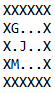
\includegraphics[width=0.5\textwidth]{figures/glue/easy.png}
        \caption{Sokoban puzzle}
        \label{subfig:easy_puzzle}
    \end{subfigure}
    \begin{subfigure}[t]{0.79\textwidth}
        \centering
        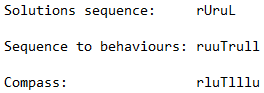
\includegraphics[width=0.6\textwidth]{figures/glue/sequences.png}
        \captionsetup{width=0.9\textwidth}
        \caption{The sequences to solve the sokoban puzzle shown in Figure \ref{subfig:easy_puzzle}.}
        \label{subfig:easy_sequences}
    \end{subfigure}
    \caption{A sokoban puzzle with a sequences of action to solve it. The "Solutions sequence" is the sequence from the path planner. The "Sequence to behaviours" is the path planner sequence converted to behaviours. The "Compass" is the behaviours sequence adjusted to the robots movement.}
    \label{fig:easy}
\end{figure}

\end{document}